\documentclass[12pt,a4paper]{article}
\usepackage[utf8]{inputenc}
\usepackage{graphicx}
\usepackage{geometry}
\usepackage{titlesec}
\usepackage{hyperref}
\usepackage{xcolor}
\usepackage{fancyhdr}
\usepackage{tcolorbox} % For colored boxes
\usepackage{multicol} % For multi-column layouts
\usepackage{mathpazo} % Use Palatino font for better readability
\geometry{margin=1in}
\pdfminorversion=5
\pdfobjcompresslevel=3
\pdfcompresslevel=9

% Colors for hyperlinks
\hypersetup{
    colorlinks=true,
    linkcolor=blue,
    filecolor=magenta,  
    urlcolor=cyan,
    pdftitle={DamageBDD: Billion-Dollar Crypto Behemoth},
    pdfpagemode=FullScreen,
}

% Title and section formatting
\titleformat{\section}{\normalfont\Large\bfseries\sffamily}{\thesection}{1em}{}
\titleformat{\subsection}{\normalfont\large\bfseries\sffamily}{\thesubsection}{1em}{}
\renewcommand{\thesection}{\arabic{section}.}

% Custom box for emphasis
\newtcolorbox{highlighted}{colback=blue!5!white,colframe=blue!75!black,arc=4mm,boxrule=1pt}

% Header and Footer
\pagestyle{fancy}
\fancyhf{}
\lhead{\textsf{DamageBDD: Billion-Dollar Crypto Behemoth}}
\rhead{\textsf{\thepage}}
\renewcommand{\headrulewidth}{0.4pt}

\begin{document}

% Cover Page
\begin{titlepage}
    \centering
    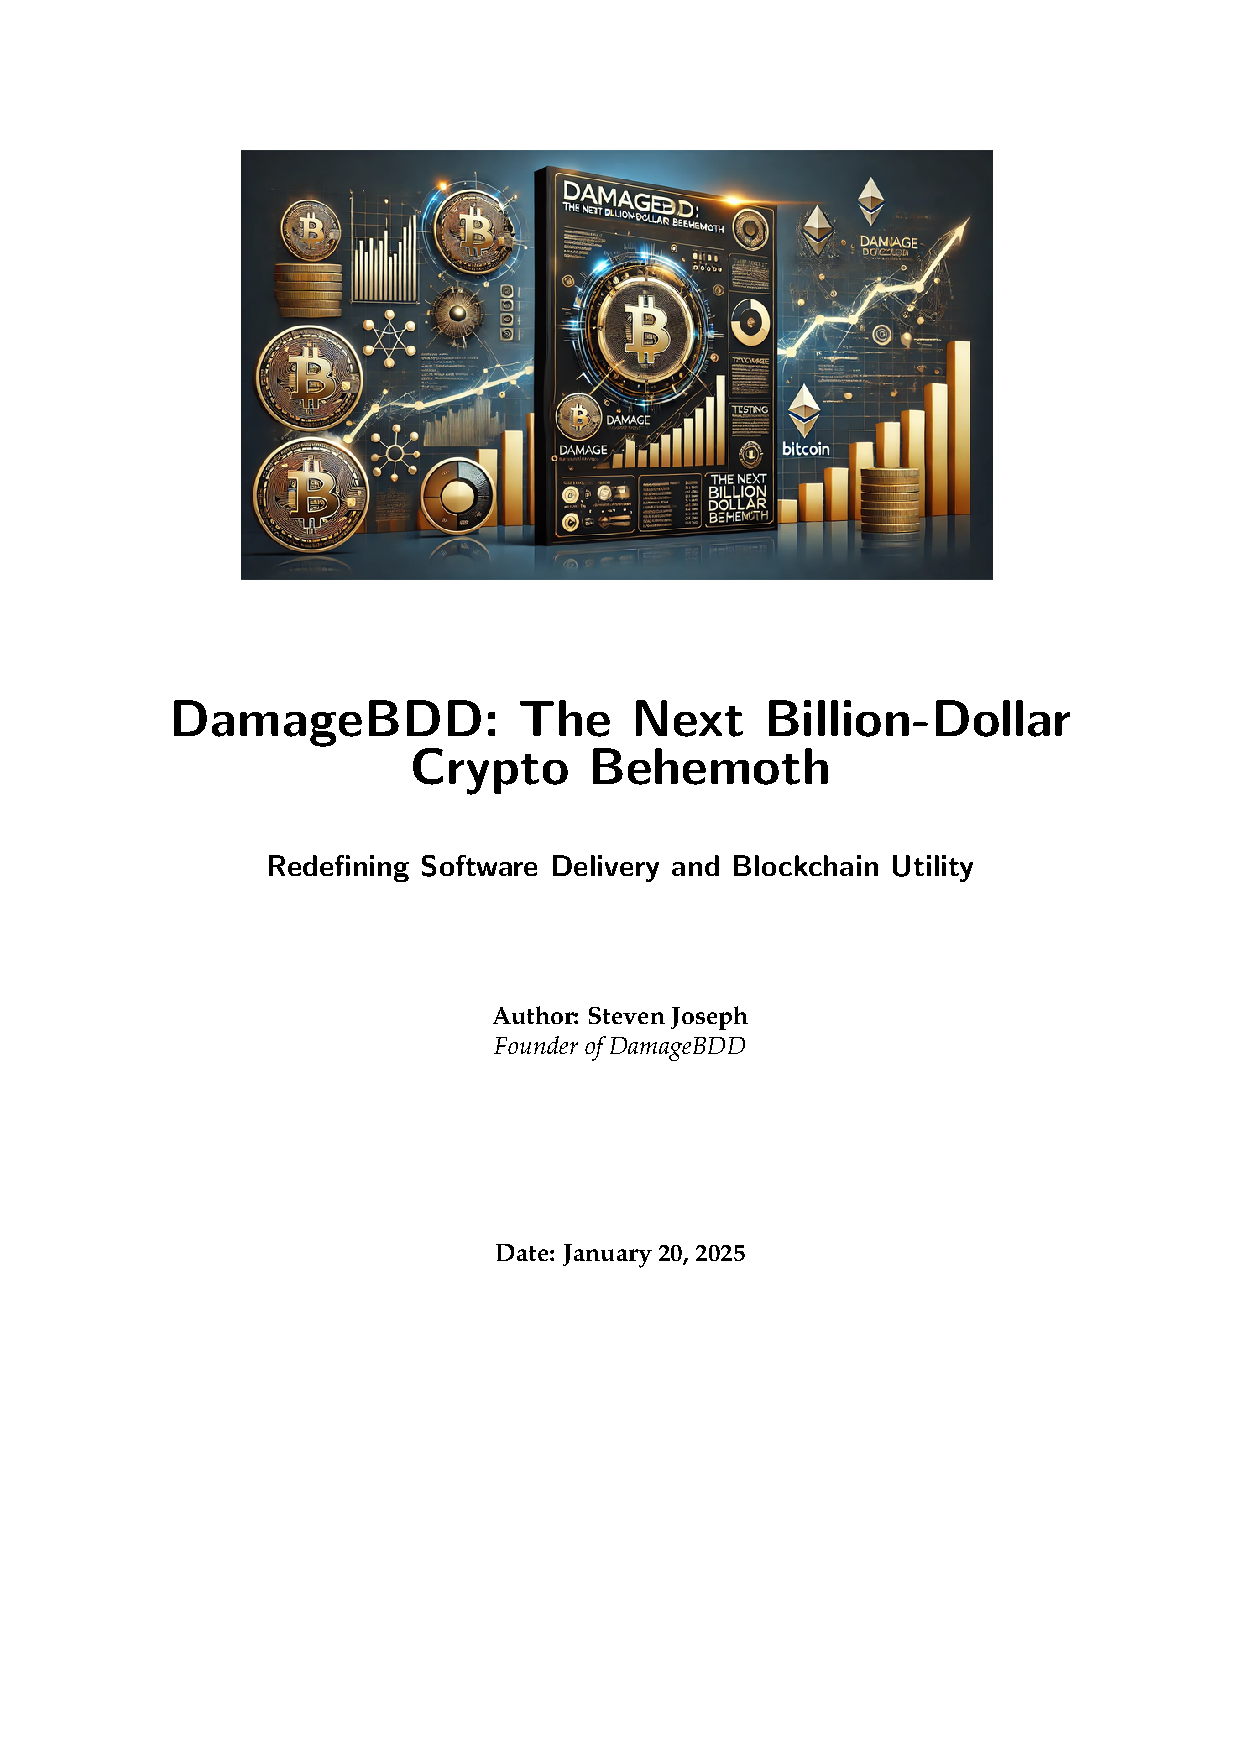
\includegraphics[width=0.8\textwidth]{compressed/billion_behemoth.png} % Replace with the path to your cover image
    \vspace{2cm}
    
    {\Huge\bfseries\sffamily DamageBDD: The Next Billion-Dollar Crypto Behemoth}\vspace{1cm}

    {\large\bfseries\sffamily Redefining Software Delivery and Blockchain Utility}\vspace{2cm}

    \textbf{Author: Steven Joseph}\\
    \textit{Founder of DamageBDD}\\
    \vspace{3cm}

    \textbf{Date: \today}\\
    \vfill
\end{titlepage}

% Abstract
\section*{Abstract}
\begin{highlighted}
DamageBDD integrates blockchain technology with behavior-driven development (BDD) to revolutionize software verification and delivery. By introducing futures and options on software milestones and leveraging Damage Tokens (DAMAGE) for incentivized participation, the platform is set to disrupt the \$30 billion software QA market. This document explores the project’s key innovations, market impact, and billion-dollar valuation potential.
\end{highlighted}

\newpage

% Table of Contents
\tableofcontents
\newpage

% Sections
\section{A Revolutionary Platform for Immutable Software Delivery}
\includegraphics[width=\textwidth]{compressed/immutable_software_delivery.png} % Replace with your image path
\begin{highlighted}
DamageBDD is the first platform to merge behavior-driven development (BDD) with blockchain immutability, creating an ecosystem where software verification becomes transparent, incentivized, and trustworthy. The introduction of futures and options on software delivery milestones adds an unprecedented layer of risk management and value creation.
\end{highlighted}

\subsection{Key Features}
\begin{itemize}
    \item On-chain BDD verification.
    \item Tokenized incentives for developers and testers.
    \item Blockchain-powered futures and options market.
\end{itemize}

\section{Damage Token: Utility Meets Liquidity}
\includegraphics[width=\textwidth]{compressed/token_liquidity.png} % Replace with your image path
\begin{multicols}{2}
The Damage Token (\$DAMAGE) serves as the lifeblood of the ecosystem, ensuring seamless incentives and liquidity. With a current value of 100 Satoshis per token and an imminent listing on Coinstore at \$0.01, it provides a compelling investment opportunity.
\end{multicols}

\subsection{Tokenomics}
\begin{itemize}
    \item 80\% reserved for founder control and scaling.
    \item 20\% released to the public at 100 tokens per Satoshi.
    \item Instant liquidity exits via the Lightning Network.
\end{itemize}

\section{Massive Addressable Market}
\includegraphics[width=\textwidth]{compressed/market_opportunity.png} % Replace with your image path
The DevOps and software QA market, projected to reach \$30 billion by 2030, is primed for disruption. DamageBDD addresses this opportunity by automating software verification and enabling risk hedging through futures and options.

\section{Competitive Advantages}
\includegraphics[width=\textwidth]{compressed/competitive_edge.png} % Replace with your image path
DamageBDD’s first-mover advantage, enterprise-grade solutions, and dual-sided network effects position it as the market leader in blockchain-based software delivery.

\subsection{Why DamageBDD Stands Out}
\begin{itemize}
    \item First platform to combine BDD verification with blockchain.
    \item Supports advanced testing frameworks like Selenium and Appium.
    \item Enables risk management via blockchain-powered futures and options.
\end{itemize}

\section{Scalability and Vision}
\includegraphics[width=\textwidth]{compressed/scalability.png} % Replace with your image path
Operating on the Aeternity blockchain, DamageBDD is designed for global scalability and seamless adoption. Future enhancements include AI-driven verification and custom risk models.

\section{Valuation Projections}
With conservative market penetration estimates, DamageBDD can facilitate \$1.5 billion in trading volume, generating \$150 million in annual fees. Combined with enterprise subscriptions and token appreciation, the platform is on track for a multi-billion-dollar valuation.

\section{Conclusion}
DamageBDD represents a paradigm shift in software delivery, combining blockchain transparency, tokenized incentives, and innovative risk management. With a visionary team and strong market fundamentals, the project is set to become a cornerstone of the crypto and software ecosystem.

\end{document}

